\section{Extended Results}
\label{app:complete}

This appendix holds the full set of models behind each main-text table, the
horizon-definition comparison, the reproduction study in detail, the Earnings25
bitrate study, the call-date-anchor variant of the post-cutoff test, and the
code-availability audit. The complete generated grids (Result Tables 1--4, every
corpus, target, metric, split and horizon) are in the separate supplement. Every
number traces to a released result CSV with a run record, and the curated tables
copy cells from those CSVs (\texttt{REPRODUCE.md} lists the command behind each).

% Stage-ladder schematic (Stage 0 -> 4, plus the reproduction track).
\begin{figure}[t]
\centering
\begin{tikzpicture}[
    node distance=3.2mm,
    box/.style={draw, rounded corners, align=center, font=\scriptsize,
                inner sep=2pt, text width=0.9\linewidth, minimum height=6mm},
    stage/.style={box, fill=black!4},
    repro/.style={box, fill=black!12},
]
\node[stage] (s0) {\textbf{Stage 0} Persistence, EWMA, HAR-RV, GARCH(1,1)};
\node[stage, below=of s0] (s1) {\textbf{Stage 1} LightGBM $+$ ticker fixed effect};
\node[stage, below=of s1] (s2) {\textbf{Stage 2} Frozen text: BGE-M3, FinBERT, surface $\to$ ridge / MLP};
\node[stage, below=of s2] (s3) {\textbf{Stage 3} Frozen audio: eGeMAPS, WavLM, emotion2vec+};
\node[stage, below=of s3] (s4) {\textbf{Stage 4} Fusion (gated / stacking)};
\node[repro, below=of s4] (sr) {\textbf{Stage R} Prior models (HTML, SCSS, KeFVP, DialogueGAT, VolTAGE) on their own data, under the same controls};
\foreach \a/\b in {s0/s1, s1/s2, s2/s3, s3/s4, s4/sr}
  \draw[->, >=stealth] (\a) -- (\b);
\end{tikzpicture}
\caption{\textbf{The modelling ladder.} From Stage~2 up, every model also carries
past-volatility covariates (and is reported with them ablated). Every stage runs
through the identity checks. The darker box is the reproduction track, which
applies the same checks to published models on their own data.}
\label{fig:pipeline}
\end{figure}


\subsection{Stages 0--3: all models}
Tables~\ref{tab:baselines}, \ref{tab:text} and~\ref{tab:audio} give the full
Stage-0/1, Stage-2 and Stage-3 model sets on the $\Delta v$ target, including the
past-volatility-only and MLP heads omitted from Table~\ref{tab:grid}.

Figure~\ref{fig:ladder} plots the canonical model of each stage from
Table~\ref{tab:grid} against the train-mean constant.

\begin{figure*}[t]
\centering
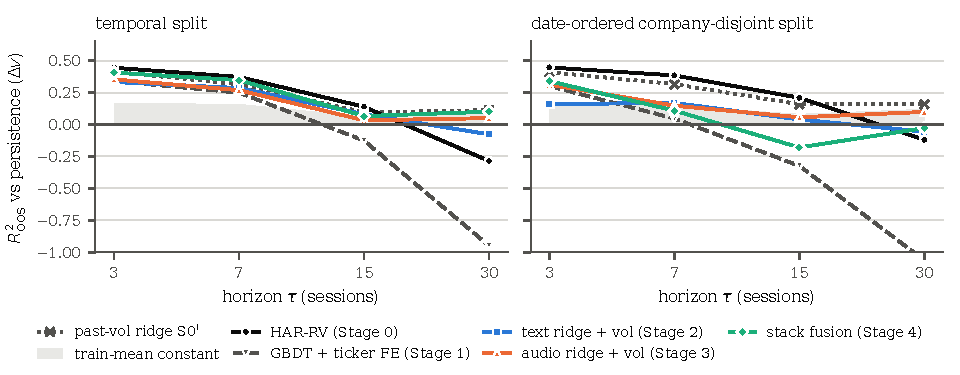
\includegraphics[width=\textwidth]{figures/fig_ladder.pdf}
\caption{\textbf{The ladder.} \Rtwo{} vs.\ persistence on $\Delta v$ (FinCall
test) for the canonical model of each stage; the shaded band is the train-mean
constant. No content stage clears HAR-RV on the temporal split, and on the
\tickerdisjoint{} split only the fusion stack does, at $\tau{=}30$. Data:
Table~\ref{tab:grid}.}
\label{fig:ladder}
\end{figure*}

% Curated headline: Stage-0/1 baselines, FinCall, Delta-v target, R^2_OOS vs
% persistence (test). Values copied from data/results/result_table_1.tex
% (temporal n=483; ticker-disjoint n=484). * = DM-significant vs persistence.
\begin{table}[t]
\centering
\small
\setlength{\tabcolsep}{4pt}
\begin{tabular}{lrrrr}
\toprule
Model & $\tau$=3 & $\tau$=7 & $\tau$=15 & $\tau$=30 \\
\midrule
\multicolumn{5}{l}{\textit{Temporal split ($n{=}483$)}}\\
Persistence       & 0.000 & 0.000 & 0.000 & 0.000 \\
EWMA              & 0.465* & 0.389* & 0.259* & 0.019 \\
HAR-RV            & 0.444* & 0.372* & 0.138* & -0.285* \\
GARCH(1,1)        & 0.472* & 0.463* & 0.298* & 0.023 \\
GBDT (ticker FE)  & 0.340* & 0.249* & -0.126 & -0.948* \\
\midrule
\multicolumn{5}{l}{\textit{Ticker-disjoint split ($n{=}484$)}}\\
Persistence       & 0.000 & 0.000 & 0.000 & 0.000 \\
EWMA              & 0.520* & 0.379* & 0.142* & 0.112* \\
HAR-RV            & 0.570* & 0.491* & 0.349* & 0.345* \\
GARCH(1,1)        & 0.561* & 0.484* & 0.334* & 0.298* \\
GBDT (ticker FE)  & 0.494* & 0.440* & 0.292* & 0.237* \\
\bottomrule
\end{tabular}
\caption{\textbf{Baselines.} \Rtwo{} vs.\ persistence on the \dv{} target,
FinCall-Surprise (test). HAR-RV is strong except on the COVID-regime temporal
$\tau{=}30$ cell. $*$: Diebold--Mariano significant vs.\ persistence ($p<0.05$).}
\label{tab:baselines}
\end{table}

% Curated headline: Stage-2 text heads, FinCall, Delta-v, R^2_OOS vs persistence
% (test). Values copied from data/results/result_table_2.tex (temporal n=483;
% ticker-disjoint n=484). * = DM-significant vs Stage-1 ticker-FE GBDT.
\begin{table}[t]
\centering
\small
\setlength{\tabcolsep}{4pt}
\begin{tabular}{lrrrr}
\toprule
Model & $\tau$=3 & $\tau$=7 & $\tau$=15 & $\tau$=30 \\
\midrule
\multicolumn{5}{l}{\textit{Temporal split ($n{=}483$)}}\\
Ridge (text)      & 0.182* & 0.202 & 0.044* & -0.133* \\
Ridge (past-vol)  & 0.412* & 0.314* & 0.094* & 0.113* \\
Ridge (text+vol)  & 0.333 & 0.285 & 0.080* & -0.077* \\
MLP (text)        & 0.013* & 0.069* & -0.253 & -1.202 \\
\midrule
\multicolumn{5}{l}{\textit{Ticker-disjoint split ($n{=}484$)}}\\
Ridge (text)      & 0.195* & 0.217* & 0.195* & 0.169 \\
Ridge (past-vol)  & 0.552* & 0.469 & 0.345 & 0.318* \\
Ridge (text+vol)  & 0.399* & 0.375 & 0.256 & 0.301 \\
MLP (past-vol)    & 0.577* & 0.508* & 0.381* & 0.356* \\
\bottomrule
\end{tabular}
\caption{\textbf{Text content (Stage 2).} \Rtwo{} vs.\ persistence on the \dv{}
target, FinCall-Surprise (test). The text-only head does not separate from the
past-volatility head, and adding text to past volatility does not help. Asterisks
mark Diebold--Mariano significance vs.\ the Stage-1 ticker-FE GBDT ($p<0.05$).
Full head set in Appendix~\ref{app:complete}.}
\label{tab:text}
\end{table}

% Curated headline: Stage-3 audio heads, FinCall, Delta-v, R^2_OOS vs persistence
% (test). Values copied from data/results/result_table_3.csv (temporal n=483;
% ticker-disjoint n=484) and data/results/audio_shuffle.csv.
% * = DM-significant vs Stage-1 ticker-FE GBDT (p<0.05; direction from the value).
\begin{table}[t]
\centering
\small
\begin{tabular}{lrrrr}
\toprule
Model & $\tau$=3 & $\tau$=7 & $\tau$=15 & $\tau$=30 \\
\midrule
\multicolumn{5}{l}{\textit{Temporal split ($n{=}483$)}}\\
Ridge (eGeMAPS)        & 0.163* & 0.156* & 0.059* & 0.079* \\
Ridge (WavLM)          & 0.156* & 0.148* & -0.027 & -0.008* \\
Ridge (emotion2vec+)   & 0.155* & 0.129* & 0.022* & 0.027* \\
Ridge (WavLM+past-vol) & 0.357 & 0.262 & -0.044 & 0.052* \\
\midrule
\multicolumn{5}{l}{\textit{Ticker-disjoint split ($n{=}484$)}}\\
Ridge (eGeMAPS)        & 0.203* & 0.119* & 0.137* & 0.044* \\
Ridge (WavLM)          & 0.178* & 0.192* & 0.131* & 0.026* \\
Ridge (emotion2vec+)   & 0.181* & 0.185* & 0.122* & 0.047* \\
Ridge (WavLM+past-vol) & 0.456 & 0.390 & 0.267 & 0.222 \\
\midrule
\multicolumn{5}{l}{\textit{Audio-shuffle control of WavLM+past-vol (\tickerdisjoint)}}\\
Real audio            & 0.456 & 0.390 & 0.267 & 0.222 \\
Within-ticker shuffle & 0.453 & 0.373 & 0.229 & 0.152 \\
Global shuffle        & 0.453 & 0.323 & 0.164 & 0.099 \\
\bottomrule
\end{tabular}
\caption{\textbf{Audio content (Stage 3).} \Rtwo{} vs.\ persistence on the \dv{}
target, FinCall-Surprise (test). Audio-only heads sit at zero everywhere; the
apparent gains of the past-vol-augmented head survive replacing every test call's
audio with a \emph{random other company's} call (global shuffle, bottom block), so
past volatility, not audio content, carries them. $*$: Diebold--Mariano significant
vs.\ the Stage-1 ticker-FE GBDT ($p<0.05$; read direction from the value). Full head
set in Appendix~\ref{app:complete}.}
\label{tab:audio}
\end{table}


\subsection{Horizon definition}
Table~\ref{tab:convention} compares the trading-day and calendar-day definitions of
the horizon on FinCall and MAEC, both at the level of the targets (sessions per
window, correlation between the two definitions) and at the level of the Stage-0
results (persistence MSE and HAR-RV \Rtwo{} under each definition).
% Curated: horizon convention delta (T9.1). Target-level rows copied from
% data/coverage/targets_convention_delta.csv (FinCall); baseline rows copied from
% data/results/result_table_1.tex (level-v, test, HAR-RV and persistence MSE).
% "sessions" = mean number of trading sessions inside the calendar-day window.
\begin{table}[t]
\centering
\small
\begin{tabular}{lrrrr}
\toprule
 & $\tau$=3 & $\tau$=7 & $\tau$=15 & $\tau$=30 \\
\midrule
\multicolumn{5}{l}{\textit{Targets (FinCall, calls ok under both conventions)}}\\
Sessions in calendar window (mean)  & 2.4 & 4.9 & 10.8 & 21.2 \\
Calls with $\ge$2 sessions (of 2{,}433) & 1{,}398 & 2{,}433 & 2{,}433 & 2{,}433 \\
corr$(v_{\mathrm{post}}^{\mathrm{trad}}, v_{\mathrm{post}}^{\mathrm{cal}})$ & 0.784 & 0.942 & 0.963 & 0.940 \\
corr$(\Delta v^{\mathrm{trad}}, \Delta v^{\mathrm{cal}})$ & 0.751 & 0.887 & 0.904 & 0.891 \\
\midrule
\multicolumn{5}{l}{\textit{Persistence MSE, level-$v$, temporal test (trading / calendar)}}\\
FinCall & 1.270 / 2.071 & 0.448 / 0.612 & 0.211 / 0.298 & 0.115 / 0.152 \\
MAEC    & 1.774 / 2.553 & 0.712 / 0.986 & 0.356 / 0.492 & 0.201 / 0.263 \\
\midrule
\multicolumn{5}{l}{\textit{HAR-RV $R^2_{\mathrm{OOS}}$ vs.\ persistence, level-$v$, temporal test (trading / calendar)}}\\
FinCall & 0.444 / 0.419 & 0.372 / 0.402 & 0.138 / 0.275 & $-$0.285 / $-$0.053 \\
MAEC    & 0.603 / 0.562 & 0.486 / 0.502 & 0.321 / 0.400 & 0.221 / 0.265 \\
\bottomrule
\end{tabular}
\caption{Horizon convention delta. The calendar-day windows of \citet{qin2019what}
hold $\sim$0.7$\tau$ sessions; at $\tau{=}3$ 43\% of the calls have at most one
post-call session and are excluded. Persistence MSE (the leaderboard's metric)
rises by 44--63\% at $\tau{=}3$ under the calendar convention, so published MSE
values are not comparable across conventions; the FinCall temporal $\tau{=}30$
deficit of HAR-RV against persistence (the COVID-regime cell, \S\ref{sec:results})
holds under both conventions ($-$0.285 / $-$0.053). Full model $\times$ horizon views under both
conventions: \texttt{data/results/result\_table\_1.tex}.}
\label{tab:convention}
\end{table}


\subsection{Reproduction study}
\label{app:repro}
Table~\ref{tab:repro} is the first entry of the study, the HTML head over our
frozen BGE-M3 chunk sequences on EC under the published split, a gapped split and
a \tickerdisjoint{} split with identical labels. Table~\ref{tab:faithful} reruns
the five papers with usable code on their own data with the authors' code wherever
it runs and a line-by-line port where it cannot. The released fidelity ledger
records every patch and substitution. Table~\ref{tab:repro-controls} gives the
absolute values behind Table~\ref{tab:repro-main}, and Table~\ref{tab:code-audit}
the code-availability audit of the seventeen papers.

\textbf{Same-Company-Same-Signal} reproduces. Its TSMixer baseline matches the 76
published cells to a median $10^{-5}$ from the shipped data alone. Its TMLP text
model on the authors' OpenAI embeddings matches per-window means within 0.03 and
recovers the paper's finding that embeddings swapped within a company do as well
as the real ones. Its training-free baselines on EC and MAEC reproduce all 48
published cells at the notebook's rounding. \textbf{HTML} does not. The released
driver splits features and labels with three independent unseeded shuffles. With
the authors' model classes unchanged on rebuilt inputs, the published recipe (ten
epochs, learning rate $2{\times}10^{-5}$, raw log-volatility targets) beats the
published number only at $\tau{=}3$ and $\tau{=}7$ on the shipped code's random
split with dropout 0, reaches the published 15- and 30-day values on no split, and
on the VolTAGE split every later paper inherited it is worse than persistence at
every horizon except $\tau{=}3$. Its text$+$audio row reproduces under the shipped
code's random split and under no other. \textbf{Sawhney et al.} cannot run as released (an unshipped call
inventory, price files and lexicons, and a TensorFlow~2.1 stack). Ported, the
finance SVR alone gives 0.712/0.370/0.218/0.154, the text and audio branches are
untrained after the two and one epochs the scripts prescribe, and the published
ensemble is reproduced only when the mixing weights are chosen on the test set, as
the released script does, where an untrained branch's near-constant output acts
as an intercept on the finance branch.
\textbf{DialogueGAT}'s corpus and labels were never released. Ported onto
FinCall's speaker turns under the paper's per-year protocol, it beats persistence
at short horizons and collapses on the 2020 split. \textbf{KeFVP}'s released
script needed five release-defect patches before it would start. Its MAEC rows use
sentence embeddings regenerated with the authors' own generator because the
released ones were never published, and seven of eight cells fall within one
published standard deviation (the eighth, MAEC-16 at $\tau{=}15$, is the row of
their table that does not average to its own stated mean). On EC the released
KePt embeddings are unavailable upstream (the linked folder is empty). With
BERT-large pooler embeddings from the same generator, which is KeFVP without its
knowledge-enhanced pre-training, the mean test MSE is 0.651/0.302/0.194/0.127
against the published 0.610/0.291/0.183/0.114, above all four published means and
within one of our repeat standard deviations at only two horizons, so the row is
not counted as reproduced.

Under the checks, the 30-session gap removes half to two thirds of KeFVP's MAEC
training calls, so those rows cannot separate leakage from data loss and are left
to the ledger. DialogueGAT's port (one seed, 42--60 held-out calls per year) shows
no consistent direction under either check.

% Curated from data/results/result_table_6r.csv (run 20260909T223252Z-reproduce-html-1ac22d6e). Numbers change only through the repository.
\begin{table*}[t]
\centering
\small
\begin{tabular}{llrrrr}
\toprule
Condition (EC) & model & $\tau$=3 & $\tau$=7 & $\tau$=15 & $\tau$=30 \\
\midrule
paper, published split, published labels & HTML (text, WWM-BERT) & 1.175 & 0.372 & 0.153 & 0.133 \\
\midrule
published split, published labels & HTML head (BGE-M3) & 0.769 & 0.436 & 0.285 & 0.223 \\
 & persistence & 1.485 & 0.570 & 0.340 & 0.202 \\
published split, our labels & HTML head (BGE-M3) & 0.760 & 0.420 & 0.285 & 0.214 \\
 & persistence & 1.826 & 0.590 & 0.333 & 0.183 \\
\midrule
embargoed temporal, our labels & HTML head (BGE-M3) & 0.778 & 0.448 & 0.278 & 0.265 \\
 & persistence & 1.948 & 0.629 & 0.353 & 0.192 \\
\tickerdisjoint{}, our labels & HTML head (BGE-M3) & \textbf{0.773} & \textbf{0.503} & \textbf{0.394} & \textbf{0.291} \\
 & persistence & 1.670 & 0.728 & 0.418 & 0.213 \\
\bottomrule
\end{tabular}
\caption{\textbf{Reproduced prior model under leakage-proof evaluation.} The HTML head reproduces the paper's ordering against price
baselines at $\tau{=}3$ and beats the published number there, but not the published
$\tau{=}15$ and $\tau{=}30$ values, which lie below the persistence floor of the
shipped labels themselves. At $\tau{=}30$ every condition is worse than
persistence. Moving the same head and labels from the published split to a
\tickerdisjoint{} split raises test MSE by 2\%, 20\%, 38\% and 36\%. The embargoed
temporal split costs 2\%, 7\%, $-$2\% and 24\%.}
\label{tab:repro}
\end{table*}

% Curated from data/results/result_table_6r_{html_faithful,scss_tsmixer,scss_tmlp,scss_aug,sawhney,
% kefvp,dialoguegat}.csv (T6R.3; run ids in docs/faithful_ledger.md). Test MSE; "ours" is
% the authors' code on the authors' data unless marked port. Persistence = past_tau.
\begin{table*}[t]
\centering
\scriptsize
\setlength{\tabcolsep}{3pt}
\begin{tabular}{llrrrrrrrr}
\toprule
& & \multicolumn{4}{c}{ours} & \multicolumn{4}{c}{published} \\
\cmidrule(lr){3-6} \cmidrule(lr){7-10}
Paper / setting & what ran & $\tau$=3 & 7 & 15 & 30 & $\tau$=3 & 7 & 15 & 30 \\
\midrule
\multicolumn{10}{l}{\textit{HTML \citep{yang2020html}, EC, authors' model classes verbatim, inputs rebuilt (WWM-BERT layer $-2$), driver corrected}} \\
\quad code: random 70/10/20, dropout 0 & text & 0.660 & 0.336 & 0.253 & 0.160 & 1.175 & 0.372 & 0.153 & 0.133 \\
\quad paper: chronological 7:1:2, dropout 0.5 & text & 0.972 & 0.439 & 0.406 & 0.248 & & & & \\
\quad published split (VolTAGE), dropout 0.5 & text & 1.231 & 1.122 & 1.063 & 1.479 & & & & \\
\quad persistence on the shipped labels & n/a & 1.485 & 0.570 & 0.340 & 0.202 & & & & \\
\quad code: random 70/10/20, dropout 0 & text $+$ 27 Praat & 0.658 & 0.347 & 0.244 & 0.165 & 0.845 & 0.349 & 0.251 & 0.158 \\
\quad paper: chronological 7:1:2, dropout 0.5 & text $+$ 27 Praat & 0.876 & 0.520 & 0.291 & 0.239 & & & & \\
\quad published split (VolTAGE), dropout 0.5 & text $+$ 27 Praat & 2.701 & 1.195 & 1.436 & 1.411 & & & & \\
\midrule
\multicolumn{10}{l}{\textit{Same-Company-Same-Signal \citep{scss2024}, DEC, authors' \texttt{run.py}, per-window means over 19 rolling quarters}} \\
\quad TSMixer (price history only) & 76 cells & 0.561 & 0.252 & 0.210 & 0.257 & 0.561 & 0.252 & 0.211 & 0.256 \\
\quad TMLP on OpenAI embeddings & 76 cells & 0.608 & 0.285 & 0.215 & 0.202 & 0.587 & 0.283 & 0.211 & 0.205 \\
\quad TMLP, embeddings shuffled within ticker & 76 cells & 0.572 & 0.276 & 0.213 & 0.209 & 0.565 & 0.273 & 0.204 & 0.200 \\
\quad TMLP, embeddings shuffled across all & 76 cells & 0.646 & 0.315 & 0.259 & 0.249 & 0.637 & 0.319 & 0.255 & 0.247 \\
\multicolumn{10}{l}{\textit{Same-Company-Same-Signal, EC / MAEC, authors' notebook, training-free, augmented same-ticker earnings history}} \\
\quad EC, Aug\_STPEV & no training & 0.569 & 0.293 & 0.201 & 0.122 & 0.569 & 0.293 & 0.201 & 0.122 \\
\quad MAEC-15, Aug\_STPEV & no training & 0.443 & 0.214 & 0.130 & 0.112 & 0.443 & 0.214 & 0.130 & 0.112 \\
\quad MAEC-16, Aug\_STPEV & no training & 0.470 & 0.238 & 0.168 & 0.113 & 0.470 & 0.238 & 0.168 & 0.113 \\
\midrule
\multicolumn{10}{l}{\textit{KeFVP \citep{niu2023kefvp}, authors' \texttt{final\_series\_infer.py} (five release-defect patches), 10 repeats}} \\
\quad MAEC-15, regenerated BERT-base embeddings & text $+$ price & 0.419 & 0.185 & 0.123 & 0.086 & 0.418 & 0.187 & 0.122 & 0.087 \\
\quad MAEC-16, regenerated BERT-base embeddings & text $+$ price & 0.442 & 0.288 & 0.363 & 0.188 & 0.445 & 0.279 & 0.303 & 0.177 \\
\quad EC, regenerated BERT-large embeddings (no KePt) & text $+$ price & 0.651 & 0.302 & 0.194 & 0.127 & 0.610 & 0.291 & 0.183 & 0.114 \\
\midrule
\multicolumn{10}{l}{\textit{Sawhney et al.\ \citeyearpar{sawhney2020mm}, EC, PyTorch port of the released scripts (their labels, split, branches); 5 seeds}} \\
\quad finance SVR (30 past volatilities) & port & 0.712 & 0.370 & 0.218 & 0.154 & & & & \\
\quad text BiLSTM, their 2 epochs & port & 2.135 & 1.580 & 1.384 & 1.401 & & & & \\
\quad aligned audio, their 1 epoch & port & 6.514 & 5.295 & 5.368 & 5.130 & & & & \\
\quad ensemble, $(\alpha,\beta)$ tuned on test (theirs) & port & 0.639 & 0.298 & 0.175 & 0.102 & 0.601 & 0.308 & 0.181 & 0.119 \\
\quad ensemble, $(\alpha,\beta)$ tuned on validation & port & 0.686 & 0.324 & 0.187 & 0.117 & & & & \\
\quad persistence on their labels & n/a & 1.491 & 0.563 & 0.345 & 0.205 & & & & \\
\midrule
\multicolumn{10}{l}{\textit{DialogueGAT \citep{sang2022dialoguegat}, PyG port on FinCall turns (role-typed speakers); published cells are on their unreleased corpus}} \\
\quad FinCall 2019 (their 2015 protocol) & port & 0.694 & 0.320 & 0.206 & 0.134 & 0.453 & 0.324 & 0.190 & n/a \\
\quad \quad persistence & n/a & 1.429 & 0.566 & 0.289 & 0.139 & & & & \\
\quad FinCall 2020 (their 2016 protocol) & port & 0.621 & 0.350 & 0.392 & 0.270 & 0.455 & 0.288 & 0.181 & n/a \\
\quad \quad persistence & n/a & 1.409 & 0.335 & 0.184 & 0.101 & & & & \\
\quad FinCall 2021 (their 2017--18 protocol) & port & 0.794 & 0.344 & 0.182 & 0.082 & 0.409 & 0.289 & 0.204 & n/a \\
\quad \quad persistence & n/a & 1.301 & 0.465 & 0.225 & 0.118 & & & & \\
\bottomrule
\end{tabular}
\caption{\textbf{Reproductions with the authors' own code and data} (Result Table
6R-F, T6R.3). Every cell regenerates from one \texttt{ecvol reproduce} command, and
the fidelity ledger lists what is verbatim, patched, substituted or reason-coded per
paper. Three of the five reproduce. TSMixer matches to $10^{-5}$, TMLP within
single-seed noise (including the paper's finding that real and within-company
shuffled embeddings score alike), and KeFVP on MAEC within one published standard
deviation on seven of eight cells with regenerated sentence embeddings. On EC, whose
released KePt embeddings are unavailable upstream, the regenerated BERT-large row is
above all four published means and within one of our repeat standard deviations at
only two horizons, and is not counted. HTML's text-only recipe does not reach its
published long-horizon cells on any split, while its text$+$audio row reproduces at
$\tau\ge 7$ under the shipped-code condition (random split, dropout 0) and on no
other. Sawhney's published ensemble is reachable only when the mixing weights are
tuned on the test set, as the released code does, with untrained text and audio
branches acting as an intercept on the finance SVR.}
\label{tab:faithful}
\end{table*}

% Curated from data/results/result_table_6r_*_controls.csv; run ids in docs/faithful_ledger.md. Numbers change only through the repository.
\begin{table*}[t]
\centering
\footnotesize
\setlength{\tabcolsep}{4pt}
\begin{tabular}{lrrrrrr}
\toprule
Model / condition & $n_{\mathrm{tr}}$ & $n_{\mathrm{te}}$ & $\tau$=3 & 7 & 15 & 30 \\
\midrule
\multicolumn{7}{l}{\textit{HTML, authors' classes (EC; seeds 0--2)}} \\
\quad text, shipped-code random split (anchor) & $\approx$390 & 112 & 0.660 & 0.336 & 0.253 & 0.160 \\
\quad text, embargoed & 285 & 101 & 0.726 & 0.347 & 0.246 & 0.178 \\
\quad text, \tickerdisjoint & 386 & 109 & 0.777 & 0.522 & 0.393 & 0.291 \\
\quad \quad persistence on the \tickerdisjoint test set & n/a & 109 & 1.452 & 0.550 & 0.327 & 0.188 \\
\quad text$+$audio, anchor & $\approx$390 & 112 & 0.658 & 0.347 & 0.244 & 0.165 \\
\quad text$+$audio, embargoed & 285 & 101 & 0.684 & 0.345 & 0.232 & 0.186 \\
\quad text$+$audio, \tickerdisjoint & 386 & 109 & 0.789 & 0.500 & 0.394 & 0.281 \\
\multicolumn{7}{l}{\quad \textit{transcript shuffle, anchor split, the 97 test calls whose company has another call}} \\
\quad text, real transcript & $\approx$390 & 97 & 0.683 & 0.348 & 0.262 & 0.165 \\
\quad text, another call of the \emph{same} company & $\approx$390 & 97 & 0.693 & 0.361 & 0.269 & 0.169 \\
\quad text, a call of a \emph{different} company & $\approx$390 & 97 & 0.745 & 0.386 & 0.318 & 0.203 \\
\quad text$+$audio, real / same company / different company, $\tau{=}3$ & $\approx$390 & 97 & \multicolumn{4}{l}{0.675 / 0.692 / 0.784} \\
\midrule
\multicolumn{7}{l}{\textit{Sawhney et al., port, ensemble with $(\alpha,\beta)$ tuned on validation (EC; 5 seeds)}} \\
\quad their split (anchor) & 328 & 110 & 0.686 & 0.324 & 0.187 & 0.117 \\
\quad embargoed & 283 & 100 & 0.719 & 0.306 & 0.184 & 0.107 \\
\quad \tickerdisjoint & 383 & 109 & 0.775 & 0.416 & 0.263 & 0.161 \\
\quad \quad its own finance SVR, \tickerdisjoint & 383 & 109 & 0.700 & 0.365 & 0.256 & 0.158 \\
\midrule
\multicolumn{7}{l}{\textit{Same-Company-Same-Signal, authors' \texttt{run.py} (DEC; seed 2021; means over 19 rolling quarters)}} \\
\quad TMLP (text), paired anchor & 900 & 30 & 0.591 & 0.288 & 0.224 & 0.211 \\
\quad TMLP (text), \tickerdisjoint & 600 & 30 & 0.660 & 0.354 & 0.280 & 0.267 \\
\quad TMLP (text), embargoed (vs anchor 0.608 / 0.285 / 0.215 / 0.202) & 895 & 90 & 0.585 & 0.287 & 0.216 & 0.208 \\
\quad TSMixer (price), paired anchor & 900 & 30 & 0.519 & 0.241 & 0.206 & 0.252 \\
\quad TSMixer (price), \tickerdisjoint & 600 & 30 & 0.556 & 0.254 & 0.194 & 0.233 \\
\quad \quad persistence on the held-out calls & n/a & 30 & 1.258 & 0.457 & 0.252 & 0.224 \\
\midrule
\multicolumn{7}{l}{\textit{KeFVP, authors' script (MAEC, regenerated BERT-base embeddings; 3 repeats)}} \\
\quad MAEC-15, paired anchor & 535 & 48 & 0.470 & 0.192 & 0.145 & 0.114 \\
\quad MAEC-15, \tickerdisjoint & 353 & 48 & 0.458 & 0.199 & 0.150 & 0.113 \\
\quad MAEC-16, paired anchor & 980 & 92 & 0.416 & 0.248 & 0.347 & 0.186 \\
\quad MAEC-16, \tickerdisjoint & 661 & 92 & 0.378 & 0.241 & 0.312 & 0.178 \\
\quad \quad persistence on the MAEC-16 held-out calls & n/a & 92 & 0.622 & 0.265 & 0.170 & 0.116 \\
\bottomrule
\end{tabular}
\caption{\textbf{The reproduced models under our controls.} Each block keeps the configuration of Table~\ref{tab:faithful} and changes
only the split. Paired anchors score the unchanged model on exactly the
\tickerdisjoint{} test calls. Removing same-company history costs the three text
models 12--82\% (HTML, Sawhney, TMLP, where TMLP is worse in 16--18 of 19
quarters) and leaves both price-dominated models unchanged (TSMixer, KeFVP),
although the \tickerdisjoint{} training sets are as large (EC) or cut by the same
third (DEC, MAEC) in both groups. The 30-session embargo moves HTML, Sawhney and
SCSS by at most 13\% in either direction. KeFVP's embargoed MAEC re-splits keep
only a half or a third of its training calls, cannot separate leakage from data
loss, and are reported in the ledger rather than here. DialogueGAT (one seed,
42--60 held-out calls per year) shows no consistent direction and is also left to
the ledger.}
\label{tab:repro-controls}
\end{table*}


\subsection{Audio by bitrate on Earnings25}
Table~\ref{tab:earnings25-audio} reruns the Stage-3 audio models on Earnings25,
pooled and per bitrate stratum, with the random swap as the check.
% Curated from data/results/audio_strata_earnings25.csv and audio_shuffle_earnings25.csv
% (run 20261006T202608Z-evaluate-audio-earnings25-6b0f8941). Ridge on WavLM + past-vol,
% Delta-v target, ticker-disjoint test segment. "increment" = real minus global-shuffle
% R^2_OOS: the part of the gain attributable to the audio content of the test call.
\begin{table*}[t]
\centering
\small
\begin{tabular}{llrrrrr}
\toprule
Stratum & calls (test) & & $\tau$=3 & $\tau$=7 & $\tau$=15 & $\tau$=30 \\
\midrule
\multirow{3}{*}{All} & \multirow{3}{*}{514 (95)} & real & 0.435 & 0.328 & 0.171 & 0.220 \\
 & & global shuffle & 0.454 & 0.327 & 0.141 & 0.206 \\
 & & \textbf{increment} & \textbf{$-$0.019} & \textbf{0.001} & \textbf{0.030} & \textbf{0.014} \\
\midrule
\multirow{3}{*}{64 kbps} & \multirow{3}{*}{281 (39)} & real & 0.370 & 0.250 & 0.109 & 0.310 \\
 & & global shuffle & 0.383 & 0.266 & 0.133 & 0.303 \\
 & & \textbf{increment} & \textbf{$-$0.013} & \textbf{$-$0.016} & \textbf{$-$0.024} & \textbf{0.007} \\
\midrule
\multirow{3}{*}{$\le$24 kbps} & \multirow{3}{*}{232 (55)} & real & 0.343 & 0.328 & 0.174 & 0.145 \\
 & & global shuffle & 0.443 & 0.354 & 0.174 & 0.128 \\
 & & \textbf{increment} & \textbf{$-$0.100} & \textbf{$-$0.026} & \textbf{$-$0.001} & \textbf{0.018} \\
\bottomrule
\end{tabular}
\caption{\textbf{Audio on Earnings25 by bitrate stratum} (T9.4; $R^2_{\mathrm{OOS}}$ vs.\
persistence, $\Delta v$, ridge on WavLM + past-vol, ticker-disjoint test). The
within-ticker shuffle is the identity here (one call per company), so the global
shuffle is the control. Call counts are inventory calls with audio at that bitrate
(one call at 32\,kbps sits in neither stratum); the heads see the 475 admitted,
priced calls, and the test count is their ticker-disjoint segment. The audio
increment never exceeds 0.03, is negative in 7 of the 12 cells, and has no
consistent sign across strata; the 64 kbps stratum is not better than the
$\le$24 kbps one. Full grid (eGeMAPS, emotion2vec+, fusion, MLP heads, all
targets): \texttt{result\_table\_3\_earnings25.csv}.}
\label{tab:earnings25-audio}
\end{table*}


\subsection{Post-cutoff evaluation under the call-date anchor}
Table~\ref{tab:lookahead-assumed} repeats the post-cutoff evaluation with day~0
anchored on the call date on both sides of the cutoff, the anchor every released
label set uses. HAR-RV barely moves, but the ridge models that carry a learned
past-volatility block collapse before the cutoff under that anchor, because the
block absorbs the reaction session that the after-hours rule leaves inside the
pre-window for before-open calls. On $\Delta v$ at $\tau{=}30$ the frozen
WavLM$+$past-volatility model is the only content model whose post-cutoff
confidence interval excludes zero under the measured anchor (0.18, CI 0.14--0.24,
against HAR's 0.08; the constant also scores 0.18 there).
That is a single-quarter observation without a Diebold--Mariano test and we report
it as exploratory.
% Curated from data/results/result_table_7.csv and result_table_7_assumed.csv
% (run 20261009T174846Z-evaluate-lookahead-aba100fd; cells unchanged from 20261006T202638Z,
% which only lacked the train-mean rows). Delta-v target, R^2_OOS vs persistence.
% Each cell: measured EDGAR anchor (primary) -> call-date anchor (variant). "in" = FinCall
% temporal test (2021); "post" = 475 Earnings25 calls. Same frozen heads under both anchors.
\begin{table*}[t]
\centering
\footnotesize
\setlength{\tabcolsep}{3.5pt}
\begin{tabular}{llrrrr}
\toprule
Head & seg. & $\tau$=3 & $\tau$=7 & $\tau$=15 & $\tau$=30 \\
\midrule
\multirow{2}{*}{HAR-RV} & in & $0.44\!\to\!0.46$ & $0.37\!\to\!0.41$ & $0.14\!\to\!0.21$ & $-0.29\!\to\!-0.28$ \\
 & post & $0.60\!\to\!0.56$ & $0.54\!\to\!0.51$ & $0.35\!\to\!0.33$ & $0.08\!\to\!-0.12$ \\
\multirow{2}{*}{text + past-vol} & in & $0.33\!\to\!-1.71$ & $0.28\!\to\!-3.12$ & $0.08\!\to\!-3.62$ & $-0.08\!\to\!-0.47$ \\
 & post & $0.31\!\to\!0.28$ & $0.33\!\to\!0.27$ & $0.23\!\to\!0.15$ & $0.12\!\to\!-0.09$ \\
\multirow{2}{*}{WavLM + past-vol} & in & $0.36\!\to\!0.26$ & $0.26\!\to\!-1.02$ & $-0.04\!\to\!-2.01$ & $0.05\!\to\!-0.56$ \\
 & post & $0.50\!\to\!0.43$ & $0.43\!\to\!0.32$ & $0.15\!\to\!0.06$ & $0.18\!\to\!0.05$ \\
\multirow{2}{*}{fusion + past-vol} & in & $0.29\!\to\!-1.73$ & $0.22\!\to\!-3.13$ & $0.04\!\to\!-0.34$ & $-0.11\!\to\!-0.45$ \\
 & post & $-0.83\!\to\!-9.97$ & $0.32\!\to\!-2.29$ & $0.19\!\to\!0.02$ & $0.01\!\to\!-0.28$ \\
\bottomrule
\end{tabular}
\caption{\textbf{Anchor sensitivity.} The same frozen heads with day~0 on the
call date, the anchor of the released label sets ($\Delta v$,
$R^2_{\mathrm{OOS}}$ vs.\ persistence). Each cell reads measured $\to$ call-date.
The ordering on level-$v$ is in the CSV.}
\label{tab:lookahead-assumed}
\end{table*}


\subsection{Code availability}
Table~\ref{tab:code-audit} is the code-availability audit of the seventeen papers
in this line, regenerated by \texttt{ecvol audit code}.
% Generated from data/results/code_availability.csv (run 20261009T215347Z-audit-code-e906e5a8).
\begin{table*}[t]
\centering\scriptsize
\setlength{\tabcolsep}{3pt}
\begin{tabular}{p{3.3cm}p{1.7cm}p{2.9cm}lp{6.0cm}}
\toprule
Paper & venue & probe (date) & verdict & reason \\
\midrule
What You Say and How You Say It Matters \cite{qin2019what} & ACL 2019 & 200, 0 code files, pushed 2022-08-04 (2026-10-09) & partial & dataset released (Drive, 5-part zip); no model code in the repository \\
HTML \cite{yang2020html} & WWW 2020 & 200, 15 code files, pushed 2024-01-05 (2026-10-09) & partial & model classes run verbatim; the released driver imports TensorFlow-1 set\_random\_seed and torchtext and splits features and labels with independent unseeded shuffles; inputs (WWM-BERT .npy, Praat features) behind dead Drive links, rebuilt; run with a corrected driver \\
 Multimodal financial forecasting \cite{sawhney2020mm}  & ACM MM 2020 & 200, 112 code files, pushed 2020-10-26 (2026-10-09) & partial & TF 2.1 / Keras 2.3.1 / tensorflow-addons 0.8.3 pins; unshipped call inventory, price files and two lexicons; text-feature script returns after one record; no multi-task loss in the released code; ported line by line to PyTorch \\
VolTAGE \cite{sawhney2020voltage} & EMNLP 2020 & 200, 5 code files, pushed 2021-11-16 (2026-10-09) & partial & ships the EC split/label files (byte-identical to KeFVP's) and GCN code; embeddings as .pkl; not ported \\
 KeFVP \cite{niu2023kefvp} & EMNLP Findings 2023 & 200, 42 code files, pushed 2024-01-28 (2026-10-09) & partial & requirements.txt does not install as written; the script starts only after five release-defect patches (missing set\_seed, package init importing undefined names, a dropped class header, an unreleased `latent` package, plotting imports); MAEC embeddings never released (regenerated with the authors' generator); EC KePt pickle Drive-only \\
DialogueGAT\cite{sang2022dialoguegat} & Findings of EMNLP 2022 & 200, 6 code files, pushed 2023-06-12 (2026-10-09) & partial & MIT code, tau<=15 only; training pickle, SeekingAlpha corpus and CRSP labels never released; DGL has no wheels for torch 2.11; ported (PyG) onto FinCall turns \\
Same Company, Same Signal \cite{scss2024} & Findings of ACL 2025 & 200, 38 code files, pushed 2026-08-13 (2026-10-09) & runnable & MIT; ships DEC with features and rolling masks; PEV/STPEV to 3 decimals, TSMixer 76 cells to 1e-5, TMLP 228 cells within single-seed noise on the authors' embeddings \\
FinTrust \cite{fintrust2023} & ACL 2023 & 200, 4 code files, pushed 2024-01-22 (2026-10-09) & partial & perturbation harness + 3/7/15/30 data; complementary control axis, not a volatility model \\
Sound of Risk \cite{soundofrisk2025} & arXiv 2025 & 200, 0 code files, pushed 2025-08-26 (2026-10-09) & none & repository holds figures only, zero source files; proprietary 1,795-call corpus \\
DeFVP \cite{niu2024does} & ICME 2024 & 409 (2026-10-09) & none & repository exists but is empty (size 0 KB, never pushed; API returns 409) \\
ECHO-GL \cite{echogl2024} & AAAI 2024 & 200, 3 code files, pushed 2024-02-26 (2026-10-09) & none & README states the code 'can not run at present'; target is direction, not volatility \\
ECC Analyzer \cite{cao2024ecc} & ICAIF 2024 & no\_url & none & no code released; GPT-4 Turbo + OpenAI embeddings \\
RiskLabs \cite{cao2024risklabs} & ICAIF-workshop 2024 & no\_url & none & no code released; GPT-4/3.5 \\
NumHTML \cite{yang2022numhtml} & AAAI 2022 & no\_url & none & paper promises code; no URL given \\
GNA-Vol \cite{shi2023gnavol} & IJCNLP-short 2023 & no\_url & none & artefact URL returns 404 (checked 2026-08-23) \\
AMA-LSTM \cite{ama2024} & NAACL 2024 & no\_url & none & 10-byte stub repository, unattributed \\
AT-FinGPT \cite{atfingpt2025} & Finance Research Letters & no\_url & none & paywalled; no artefact \\
\bottomrule
\end{tabular}
\caption{\textbf{Code-availability audit of the ECC volatility literature}
(regenerated by \texttt{ecvol audit code} with a live GitHub probe on the
date shown). One of seventeen papers ships code that runs as released. Seven ship
code with a broken environment, missing data, or defects that must be repaired
before it starts (HTML's driver imports TensorFlow-1 symbols and decorrelates
features from labels, and KeFVP needs five release-defect patches). Nine ship
nothing usable. The reason column records what the faithful-reproduction sprint
(Table~\ref{tab:faithful}) did with each.}
\label{tab:code-audit}
\end{table*}

